\documentclass[../../main.tex]{subfiles}
\begin{document}

\subsection*{8.8}
Una sottile striscia metallica di larghezza $h = 2\ cm$ è percorsa dalla corrente $i = 10\ A$.\\
Calcolare il valore del campo magnetico $\vec{B}(x)$ a distanza x dal bordo della striscia (in particolare $x\gg h$) e il momento meccanico $\vec{M}$ che agisce su un piccolo ago magnetico di momento $\vec{m} = 0.1\vec{u_x}\ Am^2$ posto a distanza $x = 1\ cm$
\\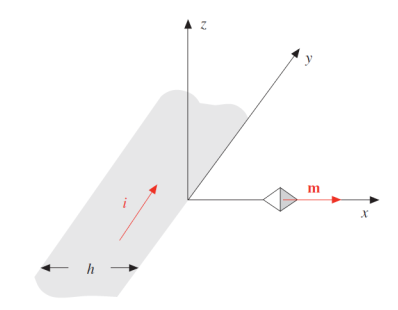
\includegraphics[scale=0.3]{e_8_8_0}
\\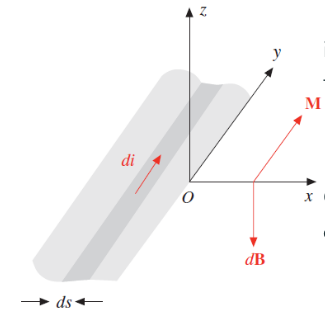
\includegraphics[scale=0.3]{e_8_8_1}
\subsubsection*{Formule utilizzate}
$\Phi\vec{B} = \frac{\mu_0di}{2\pi(x+s)}$
\subsubsection*{Soluzione punto a}
$di = \frac{i\ dx}{h}$\\
Chiamo s la distanza fra il filo e il bordo.
Quindi il campo sul ago avra direzione $-\vec{u_z}$\\
$\Phi\vec{B} = \frac{\mu_0di}{2\pi(x+s)} (-\vec{u_z})$\\
$d\vec{B} = \frac{\mu_0di}{2\pi (x+s)}(-\vec{u_z})$\\
$\vec{B} = \int d\vec{B} = \frac{\mu_0i}{2\pi h}\int_P^h\frac{ds}{x+s}(-\vec{u_z}) = \frac{\mu_0i}{2\pi h}\left[ln(x+s)\right]_{s=0}^{s=h}(-\vec{u_z})$\\
Se $x \gg h$\\
$\vec{B} = \int_0^h d\vec{B} = \frac{\mu_0i}{2\pi h}\int_0^h\frac{ds}{x+s}(-\vec{u_z}) = \frac{\mu_0i}{2\pi h}ln\left(\frac{x+h}{h}\right)(-\vec{u_z})$\\
per $x \gg h$: $\vec{B} = \frac{\mu_0i}{2\pi} \frac{1}{x}(-\vec{u_z}) = 0$
\subsubsection*{Soluzione punto b}
Da fare
\newpage

\end{document}